\section{Slacklining Variations and Categorizations}\label{3_2_slacklineVariations}
Several slackline variations originated from combining and modifying the core components of a slackline, which are the height, length, and tension~\cite{Kleindl2011-bl, MillerMauser2013-sl, Thomann2017-ab}.
Regarding the height of the slackline fixation one can differentiate between a \textit{lowline} (Figure \ref{fig:lowline}) and a \textit{highline} (Figure \ref{fig:highline}).
A lowline describes a height in which a person can safely jump off the line.
On a highline this is not possible.
Here the slacker has to make safety precautions like e.g. a seperate rope above or under the regular line in which the person can hook herself into~\cite{Kleindl2011-bl}. Hence, the majority of the lines are categorised as a lowline.
\begin{figure}[htb]
	\centering
	\begin{minipage}[t]{0.44\linewidth}
		\centering
		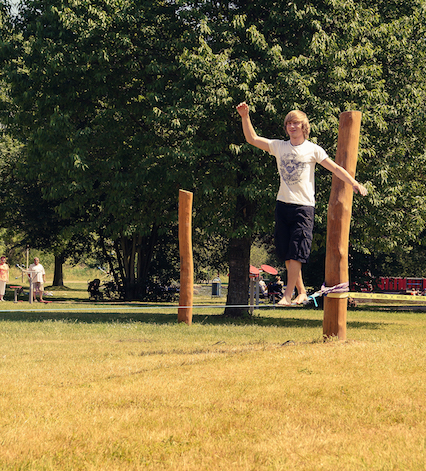
\includegraphics[width=0.94\linewidth]{Pictures/3_1_lowline}
		\subcaption{Common lowline}
		\label{fig:lowline}
	\end{minipage}
	\hfill
	\begin{minipage}[t]{0.44\linewidth}
		\centering
		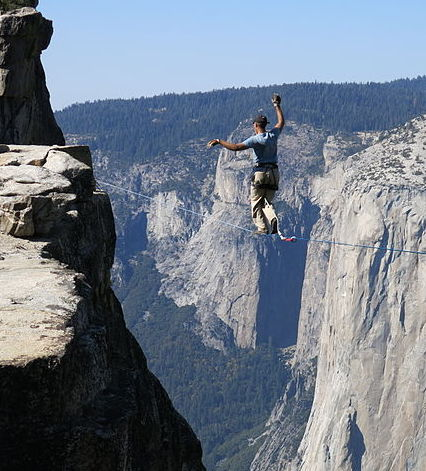
\includegraphics[width=0.94\linewidth]{Pictures/3_1_highline2}
		\subcaption{Highline between mountains~\cite{WikiSlacklining2017-lowline}}
		\label{fig:highline}
	\end{minipage}
	\caption{Main categories of slacklines}
	\label{fig:lowAndHighline}
\end{figure}

The following terms describe some fine granular variations as well as categorizations of the slackline in different application scenarios. They are not strict, which means they can differ in its scenario or can be combined with each other. A common slackline is also named \textit{trickline} (Figure \ref{fig:trickline}). It is tensioned a bit loose in about the height of the knees and has a length up to 30 m. A \textit{jumpline} (Figure \ref{fig:jumpline}) is stronger tensioned to simplify jumps on the line. It has a length of 8 - 14 m and is a bit higher than the trickline. With a \textit{rodeoline} the line is more slacked and has the highest amplitude, like seen in figure \ref{fig:rodeoline}. It is a relatively short line with a length of 5 - 8 m and the fixation points are in about 2 m such that if a person stays in the middle of the line it is just above the ground and she can swing on it sideways. Slacklines beyond 30 m are called \textit{longline} (Figure \ref{fig:longline}). The goal here is to walk as far as possible without falling off the line.

Beside these there exist some terms that describe a categorization or environment where a slackline can be applied. For example a \textit{waterline} is a line set up over a pool, sea, or a river like in figure \ref{fig:waterline}. \textit{Urbanlining} can be found, like already implied in its naming, in urban areas. Manmade buildings or structures are then used to tension the line in between, like in figure \ref{fig:urbanline}.
\begin{figure}[htb]
	\centering
	\begin{minipage}[t]{0.45\linewidth}
		\centering
		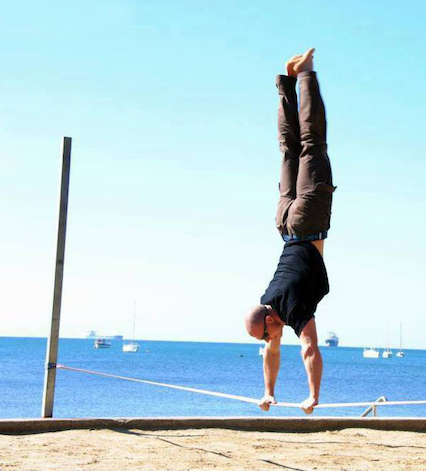
\includegraphics[width=1\linewidth]{Pictures/3_1_trickline}
		\subcaption{Handstand on a trickline~\cite{WikiSlacklining2017-trickline}}
		\label{fig:trickline}
	\end{minipage}
	\hfill
	\begin{minipage}[t]{0.45\linewidth}
		\centering
		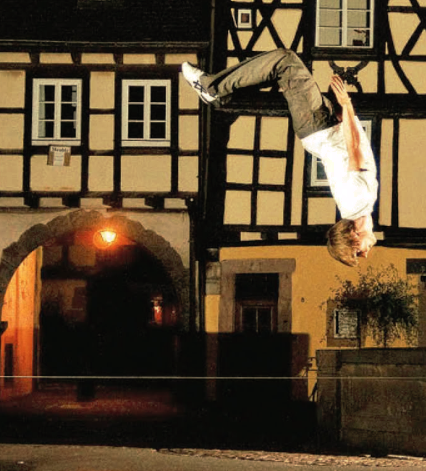
\includegraphics[width=1\linewidth]{Pictures/3_1_jumpline}
		\subcaption{Backflip on a jumpline~\cite{Kleindl2011-bl}}
		\label{fig:jumpline}
		\vspace{0.4cm}
	\end{minipage}
	\hfill
	\begin{minipage}[t]{0.45\linewidth}
		\centering
		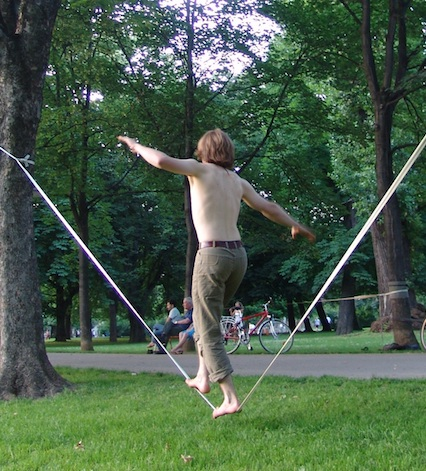
\includegraphics[width=1\linewidth]{Pictures/3_1_rodeoline}
		\subcaption{Rodeoline~\cite{WikiSlacklining2017-rodeoline}}
		\label{fig:rodeoline}
	\end{minipage}
	\hfill
	\begin{minipage}[t]{0.45\linewidth}
		\centering
		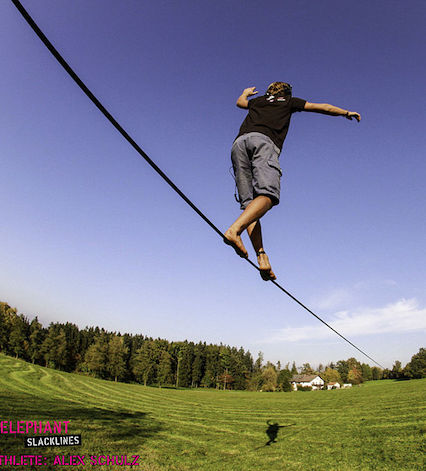
\includegraphics[width=1\linewidth]{Pictures/3_1_longline1}
		\subcaption{Longline~\cite{WikiSlacklining2017-longline}}
		\label{fig:longline}
	\end{minipage}
	\caption{Slackline variations}
	\label{fig:slacklineVariation}
\end{figure}
\clearpage
\begin{figure}[htb]
	\centering
	\begin{minipage}[t]{0.45\linewidth}
		\centering
		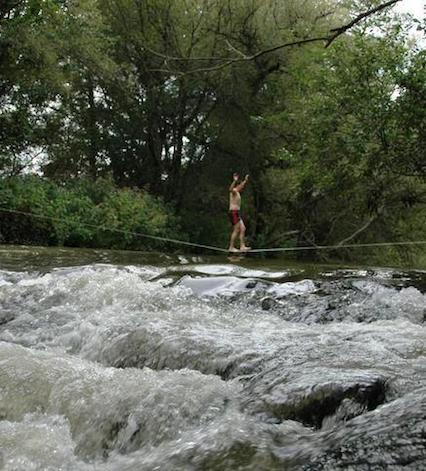
\includegraphics[width=1\linewidth]{Pictures/3_1_waterline}
		\subcaption{Waterlining over a river~\cite{WikiSlacklining2017-waterline}}
		\label{fig:waterline}
	\end{minipage}
	\hfill
	\begin{minipage}[t]{0.45\linewidth}
		\centering
		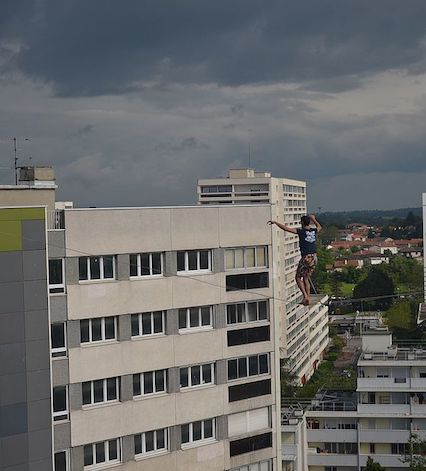
\includegraphics[width=1\linewidth]{Pictures/3_1_urbanline}
		\subcaption{Urbanlining in the city~\cite{WikiSlacklining2017-urbanline}}
		\label{fig:urbanline}
	\end{minipage}
	\caption{Categorization of slacklining}
	\label{fig:slacklineCategorization}
\end{figure}

The disadvantage of these lines is the inevitable usage of static fixation points. In the case of the SLS this would result in a constraint of variability regarding developing, testing, and study purposes. Since the focus of this thesis is mainly on beginners the slackline must not be very long. Therefore the choice felt on a mobile slackline device, which provides the needed mobility and is further described in section \textit{\nameref{5_1_technicalFeasibility}}.
